\documentclass[12pt]{article}

\usepackage[utf8]{inputenc}
\usepackage[russian]{babel}
\usepackage[T2A]{fontenc}
\usepackage{amsmath}
\usepackage{hyperref}
\usepackage{graphicx}
\usepackage[left=30mm, right=15mm, top=20mm, bottom=20mm]{geometry}
\usepackage{listings} % for code snippets

\newcommand{\high}[1]{\texttt{#1}}
% \usepackage[fencedCode,inlineFootnotes,citations,definitionLists,hashEnumerators,smartEllipses,hybrid]{markdown}


% No indentation for paragraphs
\setlength\parindent{0pt}

\begin{document}
\begin{titlepage}
\begin{center}
    Московский государственный университет имени М. В. Ломоносова

    \bigskip
    
\includegraphics[width=50mm]{msu.eps}

    \bigskip
    Факультет Вычислительной Математики и Кибернетики\\
    Кафедра Cуперкомпьютеров и Квантовой Информатики\\[10mm]

    \textsf{\large\bfseries
        КУРСОВАЯ РАБОТА СТУДЕНТА 323 ГРУППЫ\\[10mm]
        Исследование применимости алгоритма дифференциальной эволюции для процесса обучения нейронной сети
    }\\[10mm]

    \begin{flushright}
        \parbox{0.5\textwidth}{
            Выполнил:\\
            студент 3 курса 323 группы\\
            \emph{Бобко Никита Александрович}\\[5mm]
            Научный руководитель:\\
            доцент  кандидат физ.-мат. наук\\
            \emph{Попова Нина Николаевна}
        }
    \end{flushright}

    \vspace{\fill}
    Москва, 2019
\end{center}
\end{titlepage}

\newpage
\tableofcontents
\newpage

\section{Введение}

    Цель настоящей работы исследовать потенциал эволюционных алгоритмов для настройки гиперпараметров нейронных сетей. 

\section{Постановка задачи}
    Постановка задачи формулируется следующим образом: разработать алгоритм дифференциальной эволюции и попробовать обучить нейронную сеть, так чтобы она набирала как можно большее количество очков в игре Atari Frostbite.

    \subsection{Правила игры Atari Frostbite}
    Нижнии $2/3$ экрана заполнены водой с четыремя рядами ледяных глыб плывущих в горизонтальном направлении. Игрок делает свои ходы прыгая с одного ряда на другой, пытаясь избежать различных противников в виде крабов и птиц. Также есть рыбы, которые дают дополнительные очки. \\

    В верхней части экрана находится побережье, где игрок должен построить иглу. Каждый раз, когда игрок прыгает на глыбу, ряд, в котором находится глыба, меняет цвет с белого на голубой и иглу строится на $+1$ ледяной блок. После того, как игрок пропрыгал все ряды глыб на экране (напоминаем у нас всего 4 ряда ледяных глыб), то все глыбы обратно меняют цвет с голубого на белый и игрок может начать заново прыгать по глыбам. \\

    После того, как все 15 ледяных блоков, необходимых для построения иглу, собраны, игрок должен вернуться обратно на побережье и войти в иглу, это переведет игрока на следующий уровень. На каждом уровне враги и ледяные блоки двигаются быстрее чем на предыдущем уровне, тем самым усложняя игру. \\

    Каждый из уровней обязан быть закончен не более чем за $45$ секунд, иначе игрок умирает от холода. Чем быстрее закончен уровень, тем больше дополнительных очков начисляется игроку.

\section{Метод решения задачи}
    В качестве метода решения выбран алгоритм 

\section{Вычислительный эксперимент предложенного алгоритма}

\section{Описание программной реализации}
    Программная реализация построена на базе \\
    \url{https://github.com/uber-research/deep-neuroevolution}. \\
    Мою программную реализацию можно найти по адресу \\
    \url{https://github.com/nikitabobko/deep-neuroevolution}. \\
    Программа выполнена на языке Python~3.\\

    Основные модули и их описание:
    \begin{itemize}
        \item \verb!es_distributed/policies.py! содержит класс \verb!Policy! и его наследника \verb!ESAtariPolicy!. В этих классах реализованы политики обсчета нейронной сети и сама структура нейронной сети
        \item \verb!es_distributed/dist.py! содержит два класса \verb!CoolWorkerClient! и \verb!CoolMasterClient!. Это классы в которых описано взаимодействие основного процесса и процессов-рабочих. Взаимодействие сделано через пересылки сообщений по сокетам по TCP соединению. (процесс-мастер запускается по адресу \verb!127.0.0.1:9999!)
        \item \verb!es_distributed/es.py! содержит две основные функции \verb!run_master! и \verb!run_worker!, которые выполняют процесс-мастер и процессы-рабочие соответственно.
    \end{itemize}

    Чтобы начать процесс обучения нейронной сети нужно в коммандной строке выполнить следующую комманду: \\
    \verb!. scripts/local_run_exp.sh es configurations/frostbite_es.json! \\

    Программная реализация выглядит следующим образом: сначала запускается вышеупомянутый bash скрипт \verb!scripts/local_run_exp.sh!. В этом скрипте можно указать кол-во рабочих. Далее этот скрипт запускает функцию \verb!es_distributed.main.master!, в которой происходит fork всех дочерних процессов и поднимается сервер, через который в последствии будет идти общение мастера и рабочих. \\

    Далее мастер итерация за итерацией будет выполнять \verb!es_distributed.es.run_master!, где происходит алгоритм дифференциальной эволюции. Рабочим же распределяются задачи по подсчету кол-ва очков, которые набирает отдельно взятый индивид из популяции. \\

    Диаграмма UML, описанной реализации, выглядит следующим образом:
    \begin{figure}[h]
        \centering
        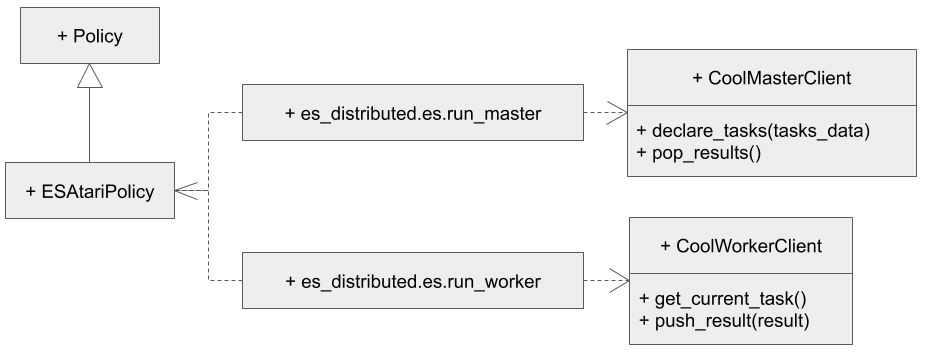
\includegraphics[width=0.8\textwidth]{uml.png}
        \caption{UML диаграмма реализации}
    \end{figure}
    
    



\section{Заключение}

\newpage
\addcontentsline{toc}{section}{Список литературы}
\begin{thebibliography}{}
    \bibitem{ConvolutionInetGuide}
    A Comprehensive Guide to Convolutional Neural Networks — the ELI5 way
    \bibitem{LiuLiu}
    Liu G. R., Liu M. B. Smoothed particle hydrodynamics: a meshfree particle method. --- Singapore : World Scientific Publishing. --- 2003. --- 449 p.
    \bibitem{DE}
    Differential Evolution (DE) for Continuous Function Optimization (an algorithm by Kenneth Price and Rainer Storn) \\
    \url{http://www1.icsi.berkeley.edu/\%7Estorn/code.html}

\end{thebibliography}

\end{document}
